\chapter{Data Analysis}
\label{ch:data_analysis}
Although we have discussed in detail the theoretical motivations for the W
physics program, as well as the machines producing the necessary collisions and
recording data produced from these collisions, we have not yet addressed the
form of the data set itself, and the substantial engineering it takes to extract
the signal of interest out of that data set.

The relative abundance of the $p + p \rightarrow W^\pm \rightarrow \mu^\pm +
\nu$ signal events is rather low, compared to the other interactions which may
take place when two protons collide. 

The previous chapter how careful triggering is employed in order to ensure that
any time this event does occur, it is recorded. This does not guarantee that
\textit{only} these events are recorded. Background events are still recored
much more frequently than signal events, even with the improved triggering. We
collected 271 $pb^{-1}$ of data (15.7 billion events, according to the PHENIX
run database) from the 2013 dataset, but there are only 3086 $W\rightarrow\mu$
events, after cuts are made (see Chapter~\ref{ch:feature_engineering}).  Of this
subset, assuming a signal to background ratio of 0.2 (this will be motivated and
described in Section~\ref{sec:sbr}), we are left with only 617 `signal events'
out of 15.7 billion total events.

This leads to the substantial problem of extracting the appropriate physics
events from the 15.7 billion event background. 

PHENIX is a multipurpose detector, and has a long history of probing a variety
of physics at a wide range of energy scales. The Muon Arms were originally
designed for the reconstruction of much lower energy charmonium dimuon decays,
and although the forward upgrade has allows us to collect most of the
$W\rightarrow\mu$ events as part of our total dataset, the task of
differentiating very high energy muons from sources of background is
challenging. Without a forward nose-cone calorimeter, or substantially more
steel absorber in place, we must resort to statistical methods to differentiate
between signal events, and background events. This is described in
Chapter~\ref{ch:feature_engineering}

\section{Raw Data to Reconstructed Parameters}

Any time a PHENIX trigger condition is satisfied, all of the information
recorded by the PHENIX spectrometer are read out from temporary on-detector
memory, and fed into a data stream that eventually is archived as a `PHENIX Raw
Data File Format' or PRDFF. 

PRDFF data is hierarchical, first being organized by event-type, and
then organized by packet-type.  There are many event types--`DATAEVENTS'
typically carry the information relevant to a physics analysis, whereas other
event-types carry very important QA information for determining the status of
the RHIC apparatus, the beam, polarization, and PHENIX performance.

Every packet has a header, which contains general information such as what the
packet contains, and in what order that packet was received. Every packet
recorded can be associated with a unique event-sequence number, which specifies
roughly the order in which the event owning the packet was received by the DAQ.
Within a given run number, an event-number is guaranteed to be unique. The
complexity of the packet is limited by the bandwidth available to move data off
PHENIX onto other storage, and the buffers/reconstruction ability of the front
end electronics modules built onto PHENIX subsystems. PHENIX archives data from
the DAQ at a rate of approximately 700 Megabytes per second--or one compact
disk.

Generally, raw PHENIX data is too complex to use straight-away, because minimal
to no reconstruction of physical properties for a certain event is done, due to
hardware limitations and time limitations--some of this raw data is often
directly used in triggering decisions, which must be made once every 106
nanoseconds or faster (the bunch crossing frequency).

The raw data collected from PHENIX undergoes a process called ``Data
Production'', where physical parameters are reconstructed from the simpler raw
data. Raw data could take any form--for example--which cathode strips were
activated in an event in the muon tracker, or, the number of photons counted in
a photomultiplier tube. This information is often combined with extensive survey
information about the geometry of a given detector, the known magnetic field in
a detector, to reconstruct quantities such as momentum, or deposited energy.

Once reconstruction has finished in a Data Production, the data are then
repackaged into ROOT files, often times internally structured into custom output
objects which are associated with a specific detector. These output objects are
simply custom C++ classes which have a serialization scheme, which have
libraries and dictionaries compiled that allow for them to be serialized into
ROOT's file format.

For the purposes of this analysis, all data has been reconstructed and
serialized into a specific type of output object called a `picoDST' or even more
concisely, `pDST'. This name, like many others in PHENIX has historical context:
DST stands for `Data Summary Tape' hearkening back to the days when data was
stored primarily on magnetic tape (it is still archived on magnetic tape!), and
`pico' because of its relatively small disk-space requirement, compared to
`nanoDST' files or simply `DST' files, which contain more granular information.

\section{Choosing Analysis Variables}


Even data reduced to the point of a pDST contains a rich and comprehensive array
of features describing the data--far more than what was ultimately used in this
analysis.  This was largely pragmatic--one can characterize the data streaming
from our detectors in many ways, and detectors themselves can be highly
granular, with each functional piece of a detector producing a stream of data.

Rather than assuming from the outset that we know which variables will provide
the most analyzing power, we observe a variety of data, and perform studies to
determine which combination of variables offers the maximum analyzing power.


The only variables which are truly relevant to this analysis need to be relevant
to understanding two questions:

\begin{enumerate}
  \item \textit{Is this reconstructed muon track the result of a real $W$ Boson Decay?}
  \item \textit{What is the polarization of the two colliding protons for every recorded collision?}
\end{enumerate}

{\noindent}To properly answer these questions, one needs to comprehensively
understand what processes are capable of producing muons, as well as whether or
not our detector can be `tricked' by signals which look like muons, but really
aren't.  Secondly, there must be a means of recovering the proton spin
polarization for each colliding bunch-pair.

The variables used in this analysis are summarized in Tables
\ref{tab:evt_variables},\ref{tab:mutr_variables}, \ref{tab:fvtx_variables} and
\ref{tab:rpc_variables}. When Cartesian coordinates are referenced, implicitly,
the reference frame is the PHENIX Coordinate system
(Figure~\ref{fig:phenix_coordinate_system}).

\section{Beam Polarization}

Polarization recovery is relatively straight-forward. Each event is uniquely
mapped to a specific colliding bunch (1,2,...,120). In turn , known `spin
patterns' are applied to each fill, which maps polarization direction to each
bunch. 

As discussed previously (Section~\ref{sec:beam_polarization}), quality assurance
apparatuses are in place to ensure the advertised spin pattern is the same as
that delivered. Since polarization patterns do not typically change in a
standard physics beam fill all that is needed is to associate a PHENIX run
number, with a RHIC fill number, and then look up the spin pattern a database.
If problems were found in the spin pattern during data taking, or later after
scrutiny, the associated data is discarded. The overall beam polarization
percentage is an important factor, which dilutes any spin asymmetry, but this is
taken into account in the final spin database QA analysis~\cite{Kim2014}, the
results of which are summarized in Section~\ref{sec:measured_beam_polarization}.

We are left with the challenging task of differentiating between signal
$W\rightarrow\mu$ events from other $X\rightarrow\mu$ events. This requires that
we engineer features from the data set which are sensitive to the difference
between signal and background. This task is challenging because the
reconstruction characteristics of our detector make it difficult to
differentiate between signal and background without employing sophisticated
statistical models to sort our data set (Section~\ref{sec:likelihood}).


\section{Data Analysis}

The thrust of the Data Analysis portion of this work is to separate the real
W-genic muons from all other muon candidates. This requires some substantial
feature engineering, creating statistical models, and a means of evaluating the
performance of these statistical models. Validating our model can be difficult
because since it requires a labeled data set. One way of model validation
employs simulating the entire data set, thus providing every muon track with a
label, and applying the statistical model to this simulated data set. This
analysis was presented in~\cite{Seidl2014a}, lending confidence to our results.

\subsection{Variables Related to Likelihood Selection}
\label{sec:analysis_variables}

In the first stage of the analysis, the variables used are: DG0, DDG0, DCA$_r$,
$\chi^2$, Rpc1DCA, Rpc3DCA, $fvtx_{dr \times d\theta}$, $fvtx_{d\phi}$, and
$fvtx_{cone}$. These variables are all related to track reconstruction, and were
chosen because they offer the most analyzing power in differentiating between
signal events and background events. Schematically, the variables are described
in Figure~\ref{fig:kinvar_side_view} and \ref{fig:kinvar_beam_view}. These
variables are chosen to be used in the Likelihood Event Selection, which is
described in Section~\ref{sec:likelihood}. Likelihood event selection us used as
an secondary cut on data, after the basic cut, described in
Section~\ref{sec:basic_cut}.

\begin{figure}[ht]
  \centering
  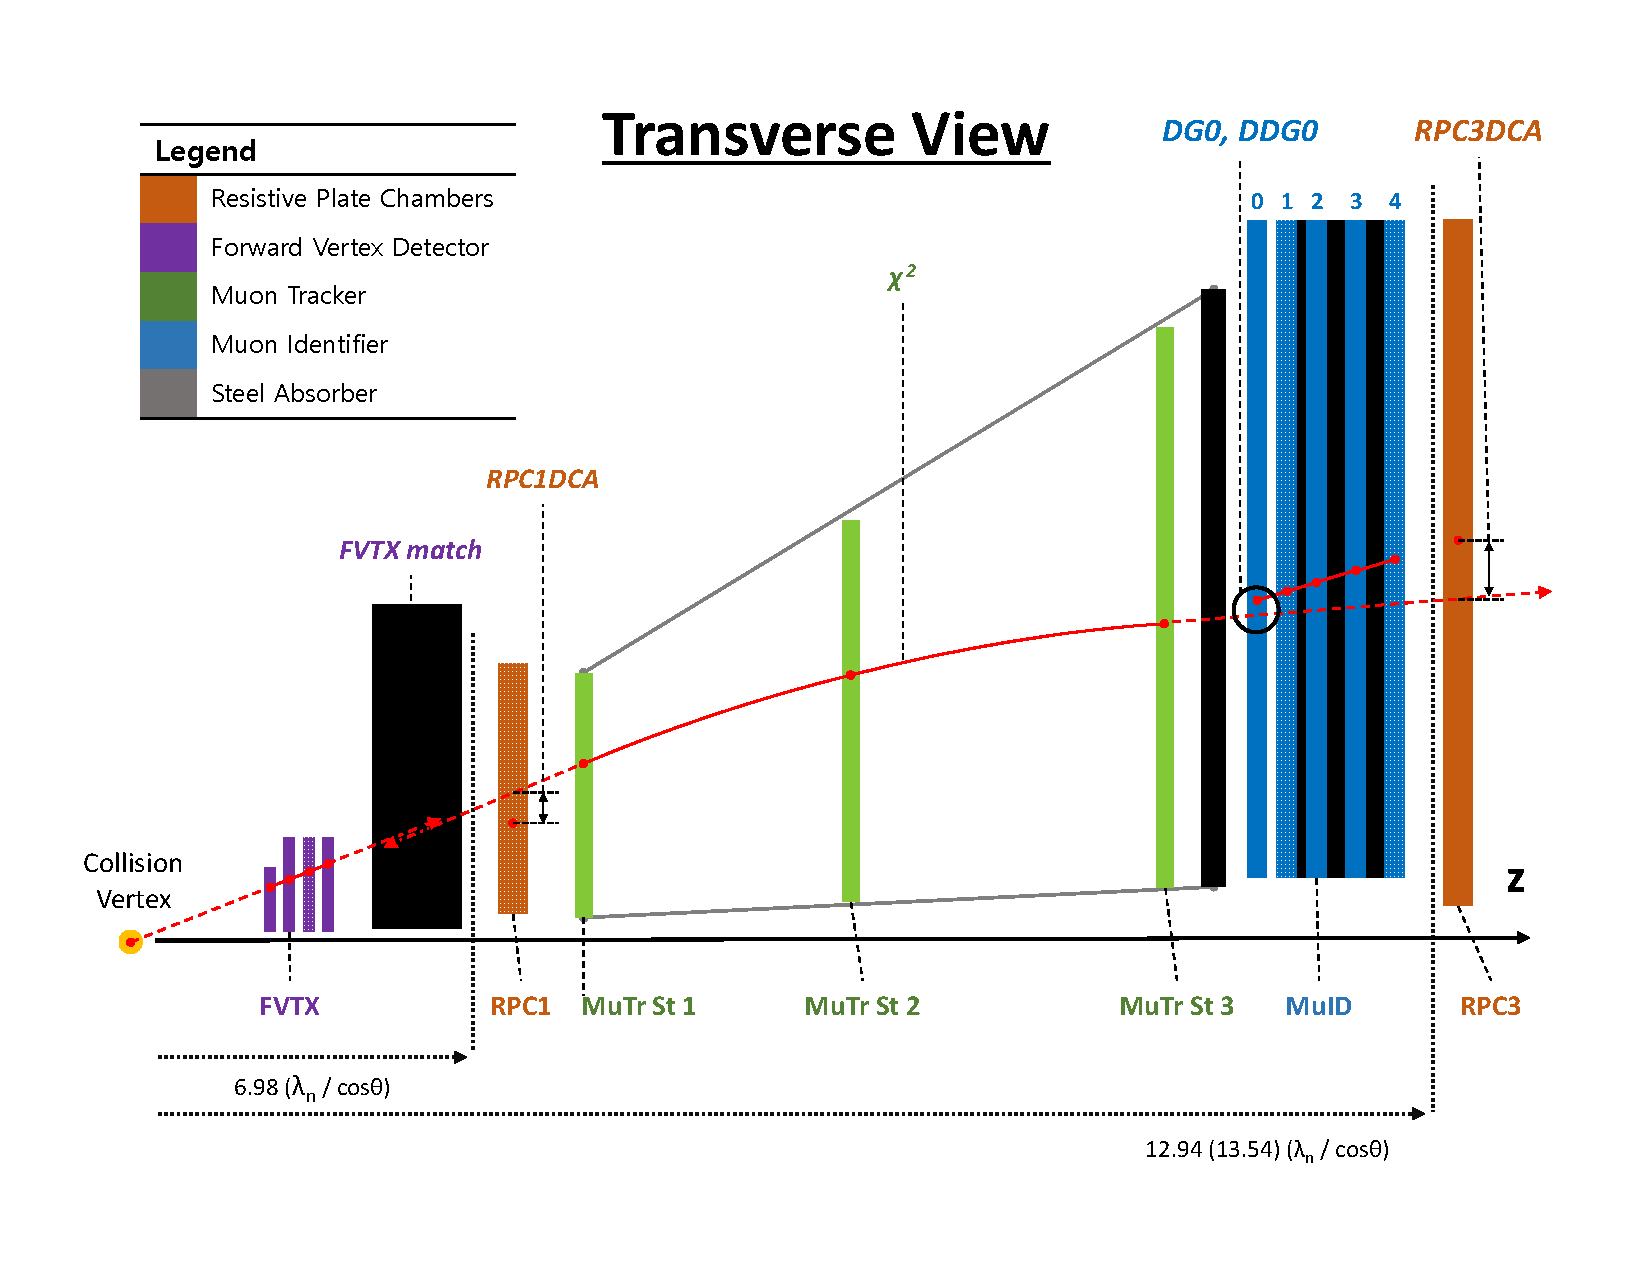
\includegraphics[width=\textwidth]{./figures/kinvar_side_view.pdf}
  \caption{
    Shown: A transverse-view of the FVTX, RPCs, MuTR, and MUID, with
    variables engineered from track reconstruction (track shown as red arc from
    yellow collision point on left)~\cite{Kim2016}
  }
  \label{fig:kinvar_side_view}
\end{figure}
    
\begin{figure}[ht]
  \centering
  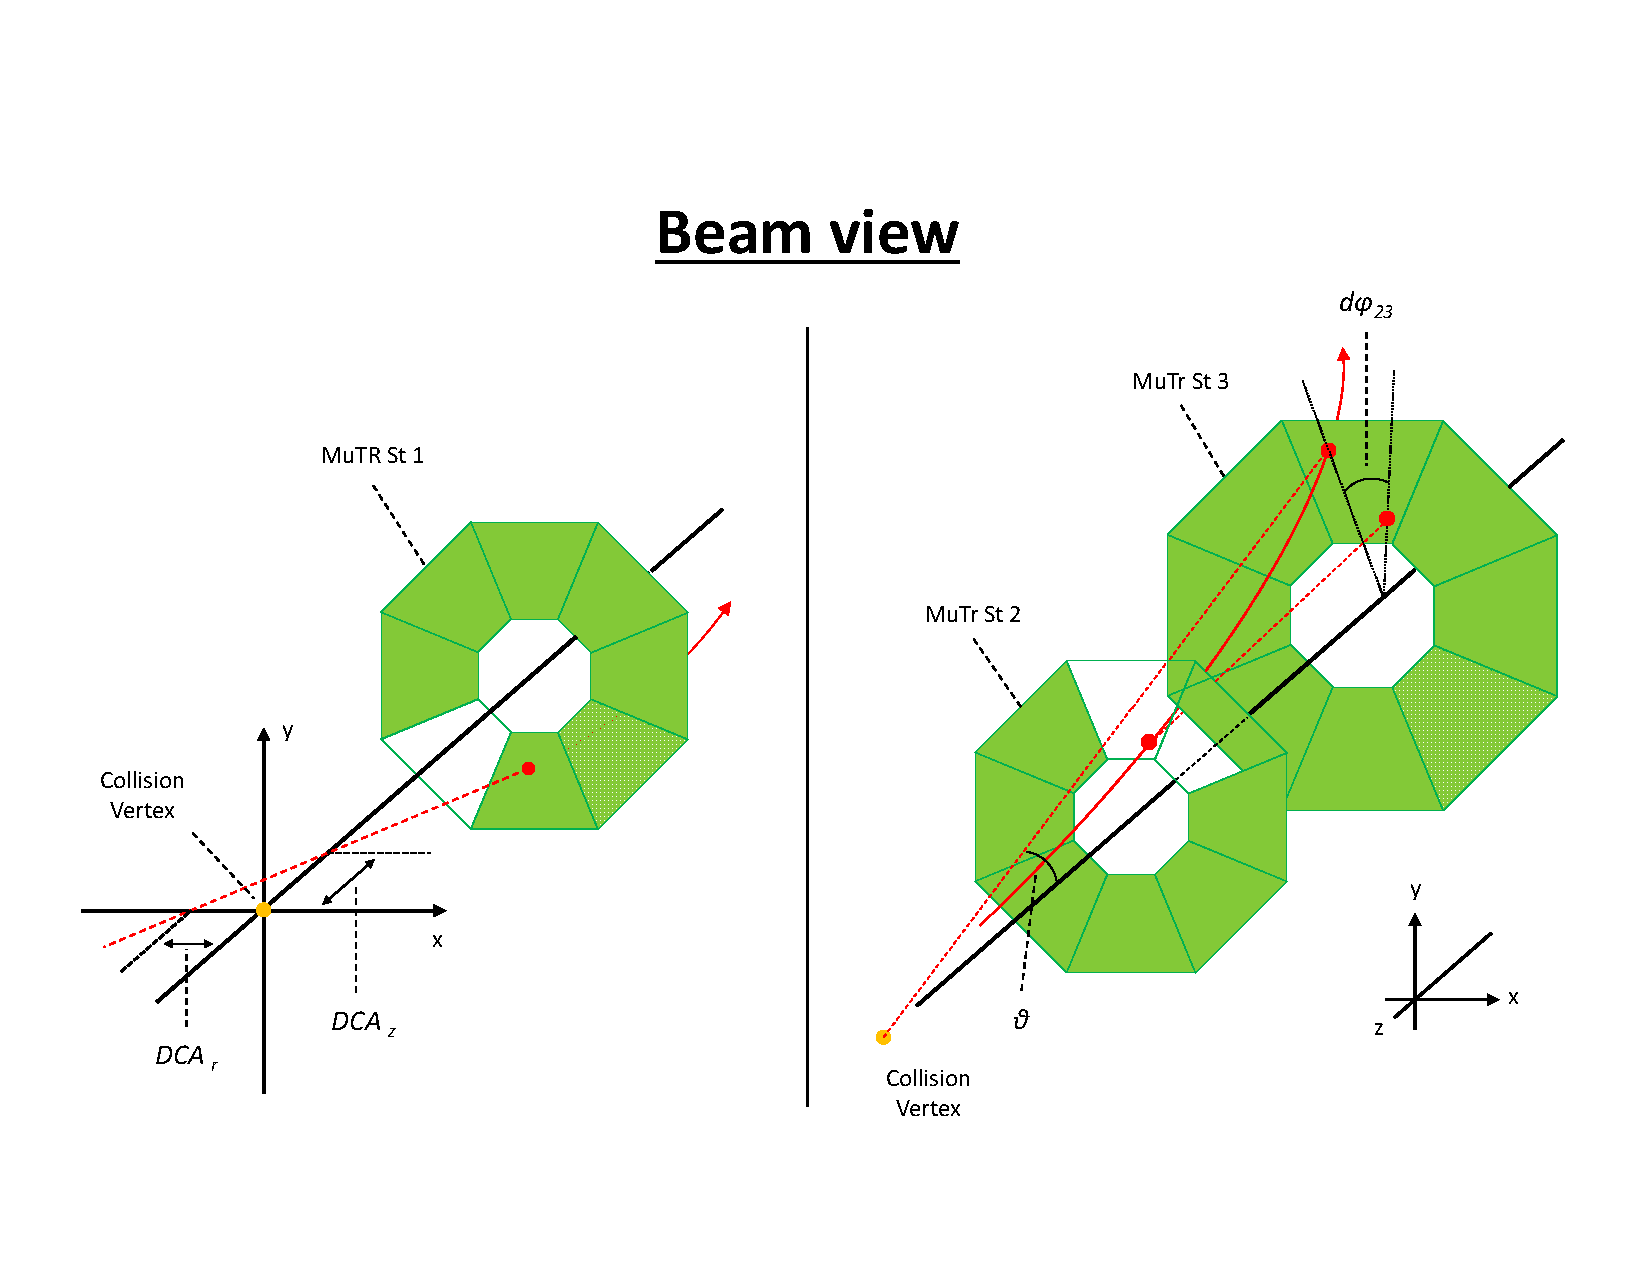
\includegraphics[width=\textwidth]{./figures/kinvar_beam_view.pdf}
  \caption{
    Shown: A beam-view of the MuTR tracking planes with additional variables
    engineered from track reconstruction~\cite{Kim2016}.
  }
  \label{fig:kinvar_beam_view}
\end{figure}

Muon tracks are reconstructed by essentially connecting the dots between `hits'
recorded at each station of the Muon Tracker.  The lines connecting these hits
are called `roads'.  Following this, the roads and hits are used to generate a
curve fit to the data, given knowledge of the muon tracker's radial magnetic
field. This curve, with knowledge of the Muon Trackers' magnetic field, is used
to obtain the charge and momentum of tracks.  Subsequently, variables are
constructed to describe the difference between the reconstructed curve, and the
`connect the dots' roads.  The smaller these differences are, the more straight
the track is, and as discussed, straightness points to higher momentum, which
ultimately leads to labeling as a W-genic particle, if the momentum is in the
correct range.

\subsubsection{DG0 and DDG0}

As seen on the left of Figure~\ref{fig:kinvar_side_view}, DG0 and DDG0
(Figure~\ref{fig:dg0_ddg0_schematic}) are variables defined relative to the
reconstructed muon track, and the road through the MUID. Concretely, the angle
that the reconstructed track makes with the road at station 0 of the MUID
defines DDG0, while the absolute distance between the track and road at MUID
station 0 defines DG0. High momentum tracks, with less bend are correlated with
both of these variables being small. Because DG0 and DDG0 are necessarily
correlated, they require special treatment in the analysis, which is described
fully in Section~\ref{sec:likelihood}.

\begin{figure}[ht]
  \centering
  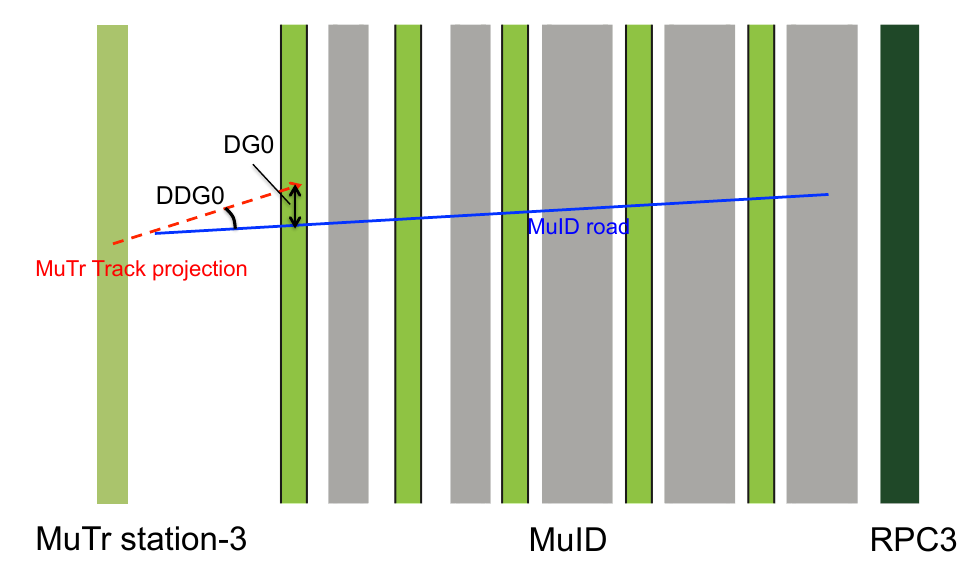
\includegraphics[width=0.7\linewidth]{./figures/dg0_ddg0.png}
  \caption{
    A schematic representation of track-matching variables DG0 and DDG0 at the
    intersection between the Muon Tracker and Muon Identifier~\cite{Oide2012}.
  }
  \label{fig:dg0_ddg0_schematic}
\end{figure}

\subsubsection{DCA$_r$, $\chi^2$, DCA$_z$}

The `distance to closest approach' (DCA$_r$) and `distance of closest approach
z' (DCA$_z$) are shown on the left of Figure~\ref{fig:kinvar_beam_view}. DCA$_r$
is defined to be the distance between the reconstructed track and the beam axis
in the transverse direction, measured at the collision vertex. DCA$_z$ is
defined similarly, except the relative distance interval is between the
collision vertex and the track's z-position at the point where DCA$_r$ is
evaluated. These
distances are useful for evaluating the reconstructed track's probable origin.
The closer to the primary event vertex, the better, as the $W$-Boson is an
interaction associated with the primary event vertex. $\chi^2$ is the reduced
chi-square associated with the quality of track fitting. The chi-square is the
resulting parameter from the Kalman filter based on the `residuals between the
measured coordinate of the cathode planes' of the Muon Tracker after taking into
account position resolution and energy losses~\cite{Oide2012}.

Because DCA$_r$ and $\chi^2$ are correlated, they require special treatment in
the analysis, which is described in Section~\ref{sec:likelihood}.
Grouped for correlation

\subsubsection{RPC Variables}
Rpc1DCA, Rpc3DCA refer to the distance of closest approach at RPC station 1 and
station 3, of the linearly extrapolated track to the closest RPC strip
associated with a hit-cluster on the RPC. These variables are shown at the
position of the RPC1 and RPC3 in Figure~\ref{fig:kinvar_side_view}.

\subsubsection{FVTX Tracking}
The Forward Vertex Detector provides additional tracking information which can
be used to identify events that originate from secondary decays, outside the
primary event vertex. $fvtx_{dr \times d\theta}$ is the product of two FVTX
tracking variables, $fvtx_{dr}$ and $fvtx_{d\theta}$. The product is taken to
reduce the dimensionality of the variable set, because the two quantities are
highly correlated. The FVTX hits are matched to the reconstructed Muon Track,
with $fvtx_{dr}$ representing the residual between the reconstructed FVTX track
and the reconstructed Muon Tracker track in the transverse direction, with
$d\theta$ and $d\phi$ representing the residuals of similar matching in the
canonical $\phi$ and $\theta$ directions. These variables are summarized in
Table~\ref{tab:fvtx_variables}.

The tracking variables discussed above all characterize the reconstruction of
muon tracks. These variables were chosen due to their sensitivity to differences
in muon tracks likely resulting from $W$-Boson decays versus other sources. This
is exploited by generating probability distributions associated with each
variable in order to calculate the likelihood of a track originating from a
signal event, or a background event, discussed in Section~\ref{sec:likelihood}.

\subsection{Variables Related to Signal to Background Ratio Extraction}
\label{sec:dataset_part_2}

In the second phase of the analysis, $dw_{23}$ and $\eta$ are employed.
$dw_{23}$ is associated with the bending of the reconstructed muon track in the
Muon Tracker volume, and is referred to as ``reduced azimuthal bending''. The
distribution of $\eta$ is expected to have distinct distribution, which differs
based on the track source--$W$-Boson decay, other real muons, and hadronic
decays in the Muon Tracker volume which are reconstructed as muon tracks. Due to
$dw_{23}$ and $\eta$ being both relatively uncorrelated to each-other, as well
as the other variables, one can avoid biasing our statistical models by
effectively over-weighting with correlated variables.

$dw_{13}$, $dw_{23}$ are shown schematically in
Figure~\ref{fig:kinvar_beam_view} and are constructed from $d\phi_{13}$, and
$d\phi{23}$.  $d\phi_{ij}$ is taken as the azimuthal bending of the track
between stations $i$ and $j$. 


\noindent$\phi_{i}$ is calculated from the $x$ and $y$ coordinates of tracks
passing through Station $i$ of the Muon Tracker:

\begin{equation}
  \phi_i = tan^{-1}\left({ySta_i \over xSta_i}\right)
  \label{eq:phi_definition}
\end{equation}

\noindent$dw_{ij}$ is constructed from $d\phi_{ij}$ as follows:

\begin{equation}
  dw_{ij} = p_T \times sin(\theta) \times d\phi_{ij}
  \label{eq:dw23_definition}
\end{equation}

{\noindent}Equation~\ref{eq:dw23_definition} is a proxy for the amount of
bending of a track between stations $i$ and $j$, which is strongly correlated to
the momentum of the track. 

A common theme amongst these variables is that they should help us distinguish
between high momentum muon tracks from $W$ Bosons, and other muon tracks. The
procedure depends on the expectation that W-genic muon tracks are kinematically
restricted to have a relatively narrow momentum distribution. Tracking variables
can be used to partially differentiate between signal and background events.

In general, W-genic events will be mostly straight, geometrically, and so this
constrains the values of variables such as DCA${}_r$ substantially, and other
variables less so. Thus, $dw_{23}$ should be a good discriminator, as it depends
on $p_T$ and the azimuthal bending of the charged tracks, due to the radial
magnetic field in the MuTR.

Our secondary requirement of our variables is that they are relatively
uncorrelated with each-other, to leave plenty of room for statistical modeling.
Ultimately, a subset of the available tracking variables are used to carry out
the analysis, in two stages. The correlation of variables for both data and
simulation are summarized in Figure~\ref{fig:kinematic_var_correlations}.

Since we are interested in recovering forward rapdity $\mu+$ and $\mu-$, and
backward rapidity $\mu+$ and $\mu-$ which result from $W$-Boson decay, we
partition the dataset into these four categories, and perform the analysis on
each category in parallel. 

The data are further subdivided based on the available track matching variables
for a given event. Not all tracking variables are available for every
reconstructed track, because not all detectors have been triggered in the same
way for every event. This is further discussed in
Chapter~\ref{ch:feature_engineering}.

\clearpage
\section{Efficiencies}
\label{sec:efficiencies}

As discussed in Section~\ref{sec:subsystems} and
Section~\ref{sec:triggering_aquisition}, particles interact with detectors, and
this interaction is transduced and used for either triggering and for
reconstructing the properties of particles. Detectors, and triggers constructed
from the transduced signals in detectors do not operate with 100\% efficiency.
A requirement for measuring cross-sections is to understand the efficiency of
these triggers and detectors, so that properly normalized yields may be measured
for various processes. The triggers used for the extraction of the
$W\rightarrow\mu$ process have been optimized to obtain the maximum signal yield
within the bandwidth allocated to the DAQ, with minimal losses due to
inefficient triggering. Due to the geometry of the detectors, the triggers used
in this analysis are more efficient in some pseudo-rapidity ranges, and less in
others. Additionally, the various triggers used for this particular analysis
(Table~\ref{tab:w_triggers}) do not share the same rapidity coverage, so the
calculation of the overall triggering efficiency is non-trivial. This analysis
of detector and trigger efficiencies are reproduced from~\cite{Seidl2014}.
Additional related plots and tables are saved for
Appendix~\ref{sec:trig_effic_appendix}.

\begin{table}[ht]
  \centering
  \begin{tabular}{r l}
    \toprule
    \textbf{Bit Number} & \textbf{Trigger Name} \\ 
    \midrule
    9 & SG3\&MUID\_1H\_N$\|$S\\
    16 & ((MUIDLL1\_N2D$\|$S2D)$\|$(N1D\&S1D))\&BBCLL1(noVtx)\\
    17 & (MUIDLL1\_N1D$\|$S1D)\&BBCLL1(noVtx)\\
    18 & RPC1+RPC3\_S\\
    19 & RPC1+RPC3\_N\\
    20 & SG3\&RPC3\&MUID\_1D\_N$\|$S\\
    21 & SG1+RPC1(C)\&MUIDLL1\_N$\|$S\\
    22 & MUON\_S\_SG1\_RPC3A\&MUID\_S1D\\
    23 & MUON\_N\_SG1\_RPC3A\&MUID\_N1D\\
    24 & MUON\_S\_SG1\&BBCLL1(noVtx)\\
    25 & MUON\_N\_SG1\&BBCLL1(noVtx)\\
    26 & MUON\_S\_SG1\_RPC3\_1\_B$\|$C\\
    27 & MUON\_N\_SG1\_RPC3\_1\_B$\|$C\\ 
    \bottomrule
  \end{tabular}
  \caption{Shown: the triggers sensitive to $W$ boson muonic
  decay~\cite{Seidl2014} }
  \label{tab:w_triggers}
\end{table}
\clearpage

\section{Rate Dependence of Detector Response}

\section{MuID hit efficiency}
In this analysis, there was a clear degradation of the MuID hit efficiency with
respect to the beam luminosity. The MuID hit efficiency is calculated based on
HV groups (described in ~\ref{Fig:efficiency:MuidEff:hvgroup}). MuID tube
efficiencies are assumed to be uniform within the same HV group.
Figure~\ref{Fig:efficiency:MuidEff:hvgroup} shows the structure of MuID HV
groups. The MuID consists of five gaps per arm, and each arm has two planes
(horizontal and vertical planes).

\begin{figure}[ht]
  \centering
  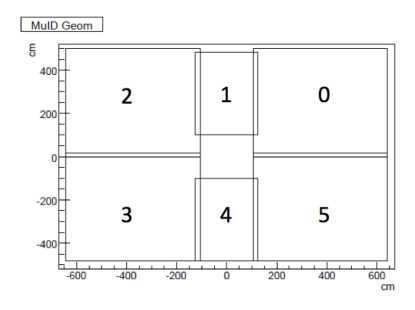
\includegraphics[width=0.75\textwidth]{./figures/muid_panel_structure.pdf}
  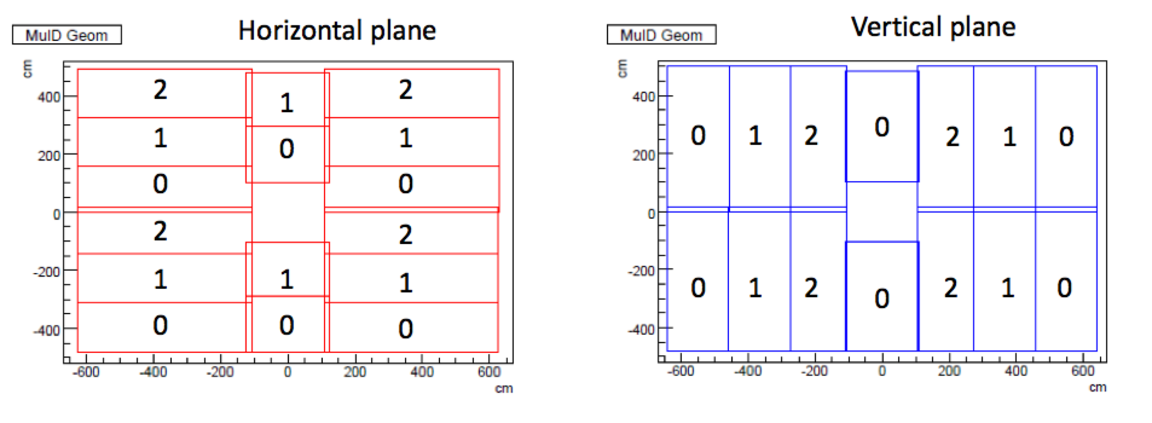
\includegraphics[width=0.75\textwidth]{./figures/muid_hv_group.pdf}
  \caption{
    The top plot shows panel numbering scheme. Each plane has six panels. The
    bottom plots show the structure of hv groups for each horizontal and
    vertical plane~\cite{Seidl2014}.
  }
  \label{Fig:efficiency:MuidEff:hvgroup}
\end{figure}

{\noindent}The MuID hit efficiency is defined as:
\begin{equation}
{\rm Efficiency_{iplane}}=\frac{\rm hit~in~iplane}{\rm MuTr~tracks~which~require~MuID~road~finder~and~trigger~emulator}
\end{equation}

{\noindent}The following cut is applied to select event samples:
\begin{itemize}
  \item Distance between MuID road and MuTr track $<$20.0\,cm
  \item Absolute $p_{z}$$>$1.3\,GeV/$c$
  \item Hits in both planes in a gap
\end{itemize}

{\noindent}An example of the MuID hit efficiency is shown in
Figure~\ref{fig:muid_first} here, with the remaining hit studies saved for the
appendix from Figure~\ref{fig:muid_first_app} to~\ref{fig:muid_last}. Hit
efficiencies are calculated for data partitioned into north or south arm,
positive or negative charges, for each gap and plane.  In all cases, the
efficiencies are compared between the 2011, 2012 and 2013 data sets.

\begin{center}
  \begin{figure}[p]
    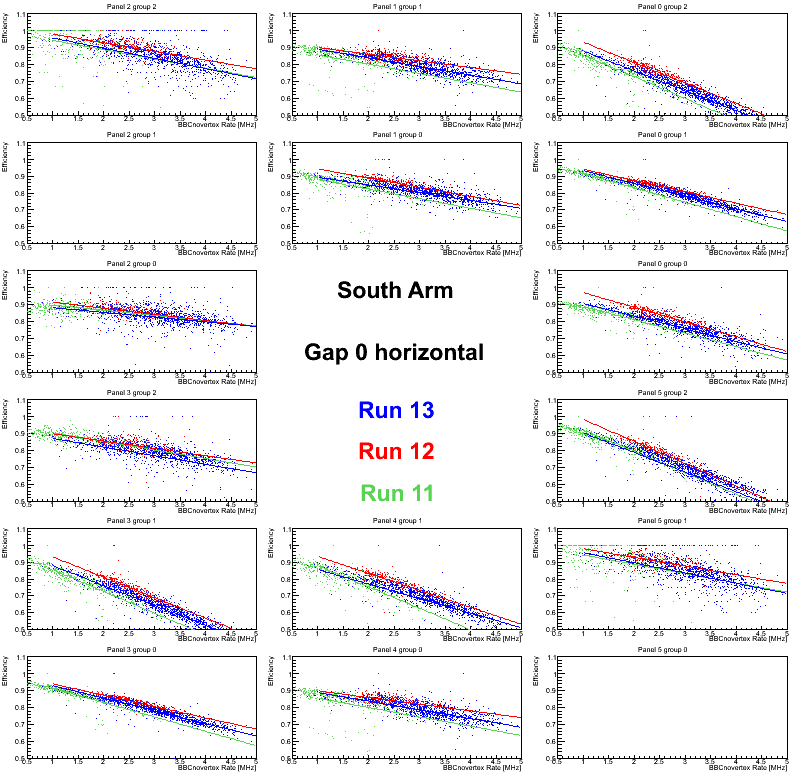
\includegraphics[width=0.99\textwidth]{./figures/efficomp_South_gap0_horizontal.png}
    \caption{
      \label{Fig:efficiency:MuIdEff:a0g0p0}MuID hit efficiency of south gap0
      horizontal plane, for the 2011 data set (green), the 2012 data set (red)
      and the 2013 data set (blue)~\cite{Seidl2014}.
    }
    \label{fig:muid_first}
  \end{figure}
\end{center}

\section{MuTR Hit Efficiency}
The MuTR hit efficiency requires some adjustment due to its discrepancy between
stereo and non-stereo planes in the same gap. The total hit efficiency is
redefined as the base efficiency used as one of the input parameters for PISA
simulation. The other parameter is the asymmetry between widths of the MuTR
planes, which is comes from the charge difference between two cathode planes in
a gap.  The luminosity dependence of hit efficiency have been determined from
the forward analyses in 2011 and 2012, and similar dependence is present in the
2013 $W\rightarrow\mu$ analysis. The method for recovering the hit efficiency
developed for the 2011 and 2012 data sets is applied for this analysis as well.
The hit efficiency is cross-checked by looking at the hit in each plane of MuTR
directly. The details of the method used in this analysis are described in
detail in~\cite{Seidl2012}.

To calculate MuTr hit efficiencies, one assumes uniform detector performance and
symmetry between two planes in a gap. Two probabilities are defined, p1 and p2.
p1 characterizes the probability of a hit in one MuTr plane `OR' another MuTr
plane, while p2 characterizes the probability that one MuTR gap does `NOT' have
a hit `OR' another gap does have a hit. Using these two probabilities, the gap
and plane efficiencies are written:

\begin{equation}
P_{k}={_n}C_{k}P_{1}^{k}(1-P_{1})^{n-k}, (0\leq k\leq n)
\end{equation}
\begin{equation}
P_{i}=\sum_{\substack{\frac{i}{2}\leq k\leq i}}{_n}C_{k}P_{1}^{k}(1-P_{1})^{n-k}{_k}C_{2k-i}(1-P_{2})^{i-k}P_{2}^{2k-i}, (k=integer, k\leq n)
\end{equation}

{\noindent}where k is the gap number, and n is the total number of gaps per arm.
Binomial fitting is performed with the above equations with respect to the plane
hit distribution to obtain the parameters p1 and p2.
Figure~\ref{Fig:efficiency:MuTrEff:hitprob} shows run by run distributions of p1
and p2 as a function of the BBC(noVtx) trigger rate.

\begin{figure}
  \centering
	\begin{subfigure}{0.5\textwidth}
		\centering
		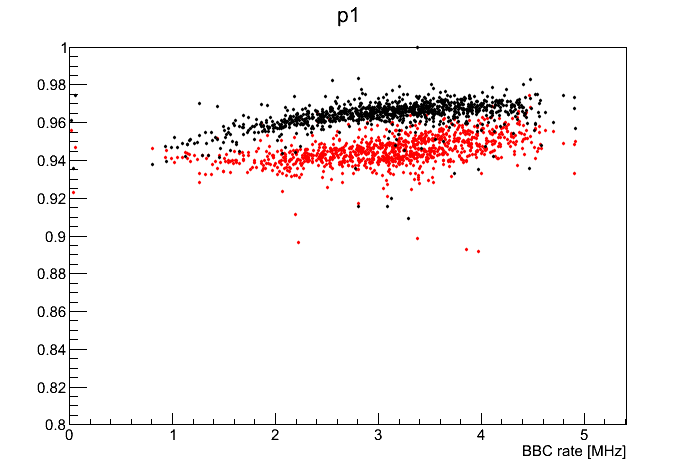
\includegraphics[width=0.9\linewidth]{./figures/mutr_hiteff_run13_p1.png}
		\caption{p1}
	\end{subfigure}%
	\begin{subfigure}{0.5\textwidth}
		\centering
		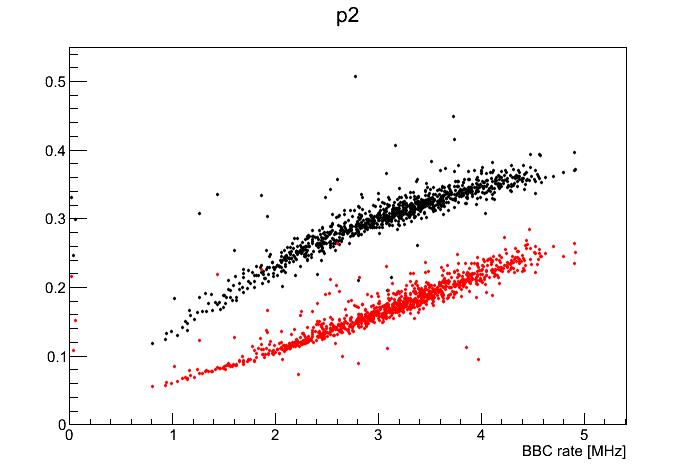
\includegraphics[width=0.9\linewidth]{./figures/mutr_hiteff_run13_p2.png}
    \caption{p2}
	\end{subfigure}
  \caption{
    Panel (a): The probability to have OR hit in a gap. Panel (b): The
    probability that a gap does not have a hit in one plane when there is OR hit
    in a gap. Both: The red points are for south arm, and black points are for
    north arm in both plots~\cite{Seidl2014}.
  }
  \label{Fig:efficiency:MuTrEff:hitprob}
\end{figure}

Gap efficiency is additionally defined to have hits in both planes and plane
efficiency using the parameter p1 and p2. The correlation between two
efficiencies becomes weaker as the luminosity increases as shown in
figure~\ref{Fig:efficiency:MuTrEff:scat}.

\begin{equation}[b]
\epsilon_{Gap}\equiv p_{1}(1-p_{2})
\end{equation}
\begin{equation}
\epsilon_{Plane}\equiv p_{1}(1-\frac{p_{2}}{2})
\end{equation}

\begin{figure}
  \centering
  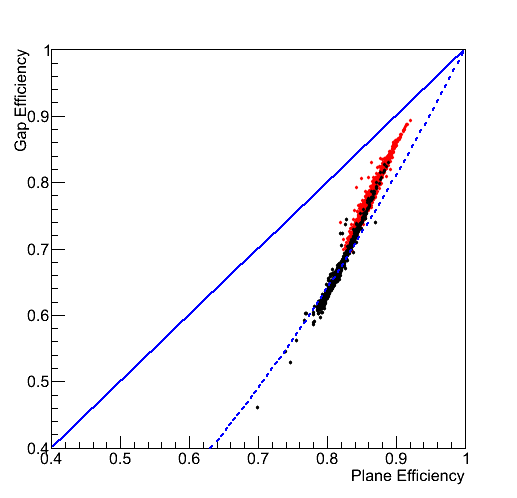
\includegraphics[width=0.5\textwidth]{./figures/mutr_hiteff_run13_scat.png}
  \caption{
    Shown: The correlation plots between gap efficiency and plane efficiency.
    The red points are for south arm, and black points are for north arm. The
    blue solid line indicates the full correlation, while the blue dashed line
    represents there is no correlation between two efficiencies~\cite{Seidl2014}
  }
  \label{Fig:efficiency:MuTrEff:scat}
\end{figure}

The parameters, base efficiency and asymmetry width are obtained, and
subsequently used to tune yields for simulations. These parameters, base
efficiency and asymmetry width additionally depend on the rate of multiple
collisions, $\mu$.

{\noindent}South Arm:
\begin{itemize}
  \item Base efficiency = 0.9725 - 0.0526$\mu$ + 0.0275$\mu^{2}$
  \item Asymmetry width = 0.3472 + 1.070$\mu$ - 1.282$\mu^{2}$ + 3.213$\mu^{3}$
\end{itemize}

{\noindent}North Arm:
\begin{itemize}
  \item Base efficiency = 0.9534 - 0.0084$\mu$ - 0.1307$\mu^{2}$
  \item Asymmetry width = 0.4322 + 0.0355$\mu$ + 3.763$\mu^{2}$ - 1.425$\mu^{3}$
\end{itemize}

\clearpage
\section{Single Muon Trigger Efficiencies}
Reconstructed muon tracks above 16 GeV in the signal region ($W_{ness} > 0.99$)
are shown in Figure~\ref{fig:triggerstack_all}, with all muon tracks plotted,
and additionally shown as relative yields in
Figure~\ref{fig:triggerrel_all}.

\begin{figure}[ht]
  \centering
  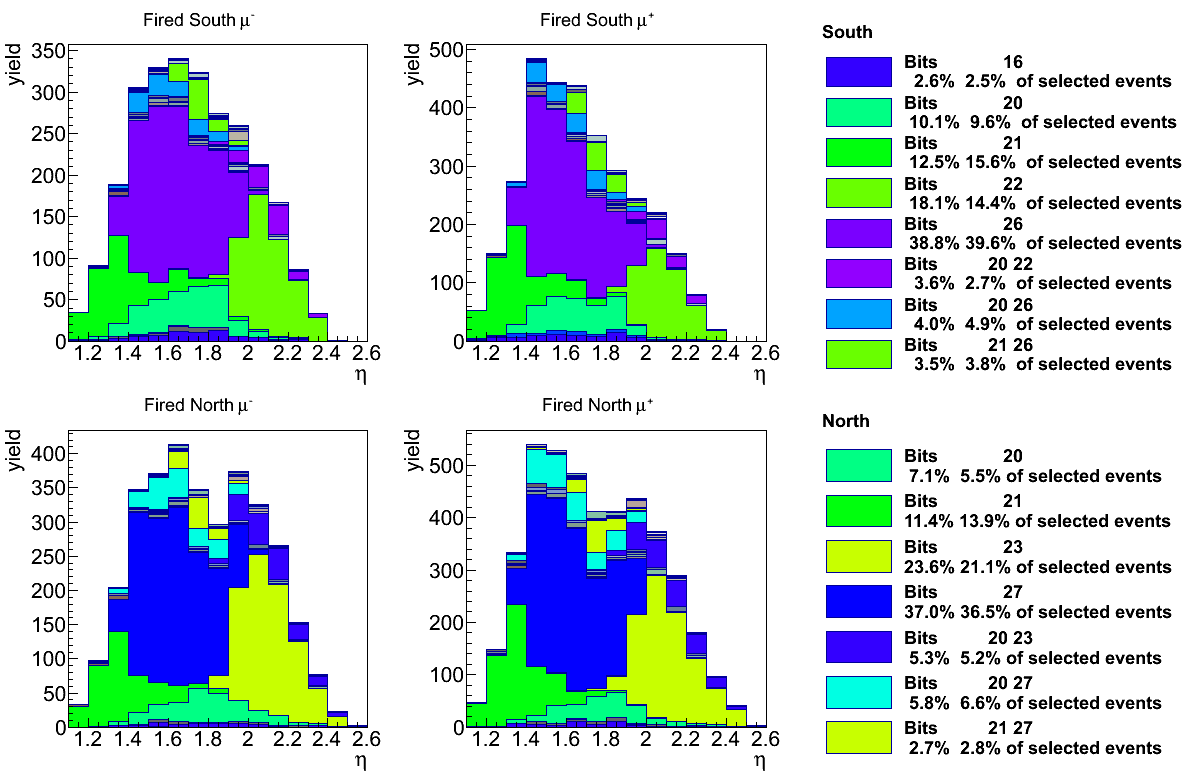
\includegraphics[width=0.8\textwidth]{./figures/triggerstack13_all.png}
  \caption{
    Shown: Absolute yields in the $W$ $\rightarrow \mu$ candidates separated by
    arm and charge for various muon triggers as a function of rapidity. Those
    with substantial contributions are given in the Legend to the right for each
    arm including their total fraction~\cite{Seidl2014}.
  }
  \label{fig:triggerstack_all} 
\end{figure}

\begin{figure}[ht]
  \centering
  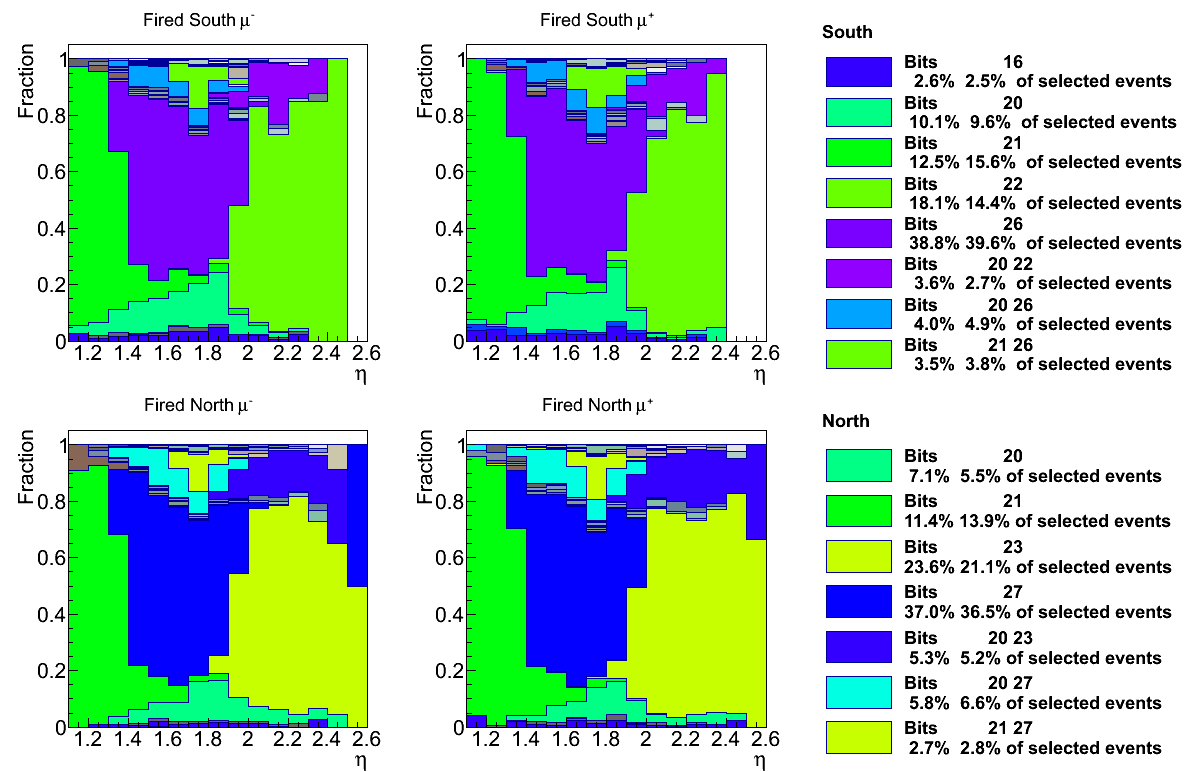
\includegraphics[width=0.8\textwidth]{./figures/triggerrel13_all.png}
  \caption{
    Shown: Relative yields in the $W$ $\rightarrow \mu$ candidates separated by
    arm and charge for various muon triggers as a function of rapidity. Those
    with substantial contributions are given in the Legend to the right for each
    arm including their total fraction~\cite{Seidl2014}.
  }
  \label{fig:triggerrel_all} 
\end{figure}

Apart from the primary physics trigger the (SG1 styled triggers,
Table~\ref{tab:w_triggers}), other triggers also contribute significantly to the
W candidate yield. These triggers are:

\begin{itemize}
  \item Trigger bit 21 (referred to as the RPC1C trigger)
  \item Trigger bits 22 and 23 (referred to as the RPC3A trigger)
  \item Trigger bit 26 and 27 (referred to as the RPC13BC trigger)
  \item Trigger bit 20 (referred to as SG3RPC3)
  \item Trigger bit 15 (referred to as 2D)
\end{itemize}

{\noindent} Furthermore one clearly sees the effect of the different trigger
acceptances related to the RPC1C, RPC13BC and RPC3A on the efficiency. As it is
common for more than one muon trigger to fire after a collision, one cannot
exclusively assign one trigger to that event. In order to obtain correct trigger
efficiencies for such events, all possible muon trigger combinations are treated
separately.  The combinatorics of this process result in 86 different
combinations for triggered events for a given muon candidate. Even so, the
majority of triggered candidates come from single or double triggers as shown in
Figures~\ref{fig:triggerstack_all} and \ref{fig:triggerrel_all}.

\section{Reference data sets and method}
In order to evaluate the trigger eficciencies for each of the trigger bit
combinations mentioned above data samples not triggered by the triggers in
question are needed. The most independent samples are those triggered either by
triggers in the MPC, triggers in the ERT or Minimum Bias triggers. These various
triggers do exist as separated streams on the Taxi and were thus directly used
to evaluate the efficiencies. 

The triggers used in the evaluation relate to:
\begin{center}
\begin{tabular}{r|l| r | r | r}
  \toprule
  \textbf{Bit} & 
  \textbf{Trigger Name} & 
  \textbf{ERT} & 
  \textbf{MPC} & 
  \textbf{Minbias} \\ 
  \midrule
      0 & BBCLL1($>$0 tubes)  & X & X & O\\
       1 & BBCLL1($>$0 tubes) novertex  & X & X & O\\
       3 & BBCLL1(noVtx)\&(ZDCN$\|$ZDCS) & X & X & O\\
       4 & BBCLL1($>$0 tubes) narrowvtx & X & X & O\\
       6 & ERT\_4x4b & O & X & X\\
       7 & ERTLL1\_4x4a\&BBCLL1(noVtx) & O & X & X\\
       8 & ERT\_4x4c\&BBCLL1(noVtx) & O & X & X\\
      10 & ERTLL1\_E\&BBCLL1(narrow) & O & X & X\\
      12 & MPC\_B & X & O & X\\
      13 & MPC\_A & X & O & X\\
      14 & MPC\_C\&ERT\_2x2 & X & O & X\\
      15 & (MPCS\_C\&MPCS\_C)$\|$(MPCN\_C\&MPCN\_C) & X & O & X\\ 
  \bottomrule
  \end{tabular}
\end{center}

{\noindent}where ``O'' corresponds to a matching trigger for that data set and
``X'' corresponds to a not matching trigger.

The trigger efficiencies for triggers which do not include the 1D triggers can
be evaluated directly, while those including the 1D triggers additionally
require the multiplication of the 1D efficiencies from the other samples. The
corresponding 1D trigger efficiency is then applied when combining all triggers
and efficiencies into a total trigger efficiency used for the $W$ candidate data
sample. 

The extraction strategy compares for each trigger bit a in question
the number of good candidate muon events with the particular trigger bit live
with the total number of good candidate muon events in the particular data
sample (Reference trigger):

\begin{equation}
\epsilon_{\mathrm{Trigger a}} = \frac{(\mathrm{muon candidate})_{\mathrm{Reference trigger}} \&\& (\mathrm{Trigger a live}) }{(\mathrm{muon candidate})_{\mathrm{Reference trigger}}}\quad.
\end{equation}

The trigger efficiencies after the Basic Cut (Section~\ref{sec:basic_cut}) can
still depend on muon rapidity, $p_T$ and $W$ likelihood ratio.
Ideally a three-dimensional binning would properly address all those potential
dependencies, but the statistics are not sufficient to evaluate the trigger
efficiencies up to the high $p_T$ and $W$ likelihood ratios
required for the final $W$ selection. Therefore various aspects are studied in
lower dimensional binning with slightly less stringent cuts. After, one
extrapolates to the signal region. Different ways of extrapolating to the region
of interest will then be compared and systematic errors on the total trigger
efficiencies will be assigned based on their comparison. 

\subsection{Rapidity Dependent Efficiencies}

The first set of efficiency studies uses a fine rapidity binning of 15
equidistant bins with $1.1<\vert\eta<2.6$ and a minimum $p_T$ of 5
GeV and a $W_{ness}$of above 0.9.  The corresponding efficiency
distributions separated by arm, charge and trigger. An example is shown in
Figure~\ref{fig:run13_trigeffieta_w0_nper0_trig16_lin}, with remaining Figures
produced in the Appendix from
Figure~\ref{fig:run13_trigeffieta_w0_nper0_trig17_lin} - to
Figure~\ref{fig:run13_trigeffieta_w0_nper0_trig27_lin}. One sees, that the 1D
trigger is mostly equally efficiency at all rapidities with maybe a hint of
decreasing efficiencies at higher rapidities. 

The same is true for the SG1 triggers (bits 24/25) which also have consistent
efficiencies.  The trigger bits 18 and 19 which are highly prescaled to reflect
the combined acceptances of the RPC1 and the RPC3. Thus, bits 18 and 19 are only
efficient from $1.4 \vert\eta\vert 2.0$ and have decreasing efficiency for
increasing rapidity. Also, the production triggers RPC13\_BC (bits 25/26) show
the same rapidity dependence and are mostly efficient over $1.4 \vert\eta\vert
2.0$.  The SG3RPC3 triggers have a flat efficiency above the acceptance edge of
the RPC3 at around $\eta\approx1.4$. This trigger is efficient without respect
to $W_{ness}$ cut, and therefore contributes a reasonable fraction of the $W$
candidate events.  The RPC1C trigger is only efficient in the RPC1 acceptance,
at $\eta < 1.4$ and conversely the RPC3A triggers are only efficient at $\eta >
2$.

\begin{figure}[ht]
  \centering
  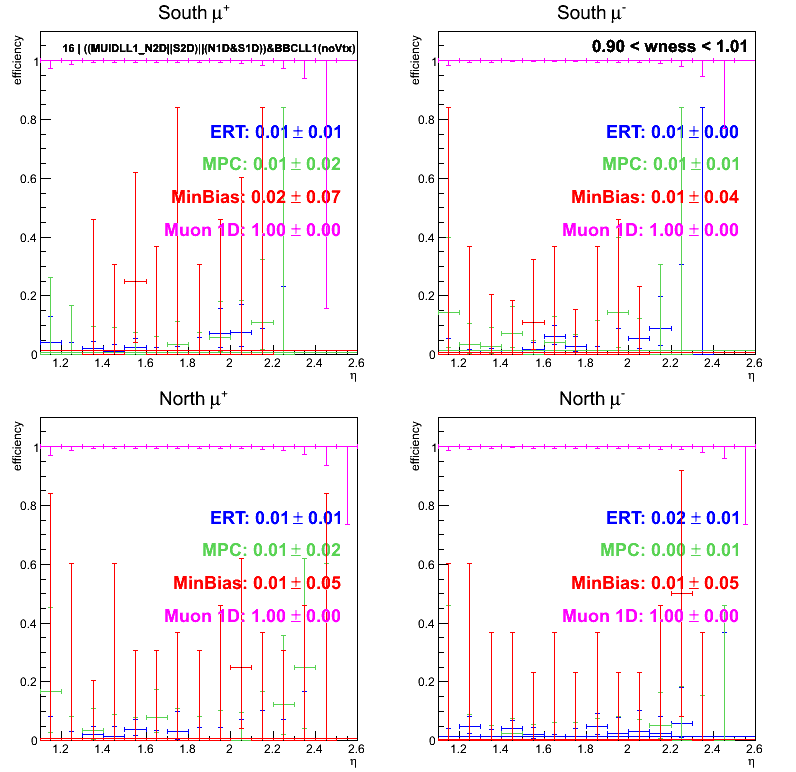
\includegraphics[width=0.8\textwidth]{./figures/run13_trigeffieta_w1_trig16_lin.png}
  \caption{
    Shown: Trigger efficiencies for trigger bit 16
    (((MUIDLL1\_N2D$\|$S2D)$\|$(N1D\&S1D))\&BBCLL1(noVtx)) for single $W$
    $\rightarrow \mu$ candidates with $p_T$ above 5 GeV. The
    efficiencies for ERT (blue), MPC (green), MinBias(red) and 1D (purple)
    triggered data samples are shown as well as a constant fit over the whole
    range~\cite{Seidl2014}.
  }
  \label{fig:run13_trigeffieta_w0_nper0_trig16_lin} 
\end{figure}

\clearpage
\subsection{$p_T$ Dependent Efficiencies}
To study $p_T$ dependent efficiencies, no $W_{ness}$ cut is
applied, though data is binned in three rapidity bins, $1.1 < \eta < 1.4$, $1.4
< \eta < 2.0$ and $2.0 < \eta < 2.6 $. Data is plotted as a function of $p_T$.
As an example, Figure~\ref{fig:run13_trigeffipt_eta0_nper0_trig17_lin} is shown
from this study, with remaining
Figures~\ref{fig:run13_trigeffieta_w0_nper0_trig17_lin}-\ref{fig:run13_trigeffipt_eta1_nper0_trig27_lin}
shown in the appendix.

Additionally, fit results are shown alongside the efficiencies. The full $p_T$
range is fitted with an error function and momentum above 10 GeV is fitted with
a constant term. With no $W_{ness}$ cut applied, the data is dominated by
hadronic background. The results of the fits will later be used as lower limits
of the total trigger efficiencies. 

\begin{figure}[ht]
  \centering
  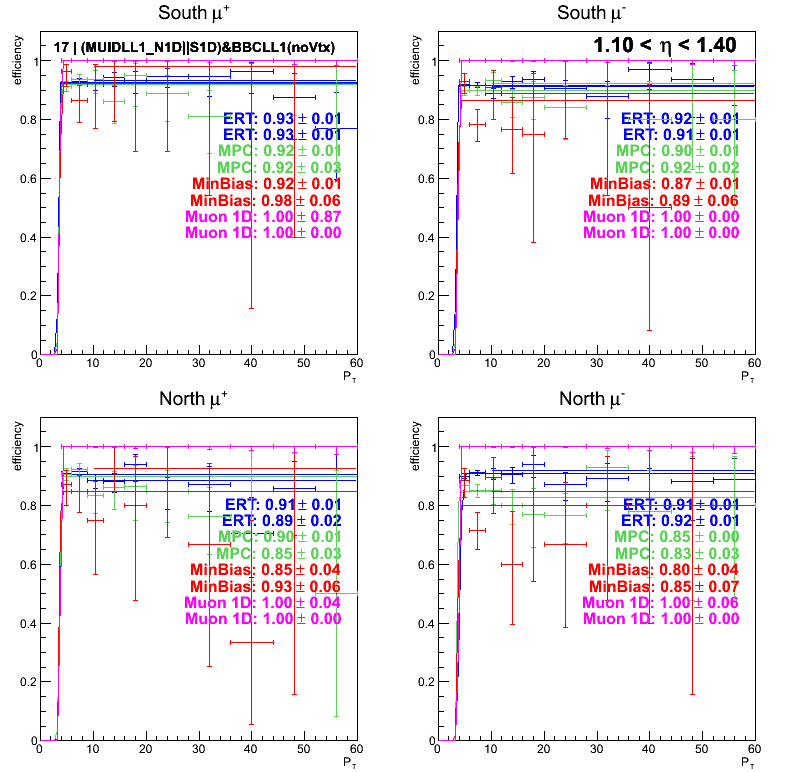
\includegraphics[width=0.8\textwidth]{./figures/run13_trigeffipt_eta0_trig17_lin.png}
  \caption{
    Trigger efficiencies for trigger bit 17
    ((MUIDLL1\_N1D$\|$S1D)\&BBCLL1(noVtx)) for single $W$ $\rightarrow \mu$
    candidates in the rapidity range $ 1.1 < \eta < 1.4$ as a function of
    $p_T$. The efficiencies for ERT (blue), MPC (green),
    MinBias(red) and 1D (purple) triggered data samples are shown as well as a
    constant fit over the whole range~\cite{Seidl2014}.
  }
  \label{fig:run13_trigeffipt_eta0_nper0_trig17_lin} 
\end{figure}

One sees very clear turn-on curves for nearly all triggers and rapidity ranges.
However, some efficiencies seem to drop again at $p_T$ above about 10 GeV. As a
consequence the constant fits to this higher $p_T$ region are generally lower
than the plateau of the error function fit. The reason for this drop can be
understood qualitatively as an effect from hadronic background mis-reconstructed
as high $p_T$ muons. As shown in \cite{Seidl2012}, at high $p_T$ the fake muons
dominate. The hadronic background tends to create a signal in the MuTR which are
associated with lower efficiencies and increased multiple scattering in the SG1
and RPC3 triggers. At $p_T$ close to the thresholds of SG1 and related triggers
the fraction of hadrons is still rather high, but they are much more likely to
be correctly reconstructed at several GeVs and thus their signals are more
likely to fire the SG1. In addition the majority of real muons can be also found
at these intermediate momenta. 

To summarize, the high momentum efficiencies seem to be lower due to the fake
muon content and the plateau results just above the thresholds are more likely
to correspond to actual muon efficiencies. However, once these fakes are removed
via the $W_{ness}$ cuts the actual efficiencies at high $p_T$
are expected to rise to at least the plateau values.  

When adding $W_{ness}$ cuts, the high $p_T$ sample is calculated to have a
higher efficiency. An example is shown in
Fig.~\ref{fig:run13_trigeffiptlowhighpt} for comparison.

\begin{figure}[ht]
  \centering
  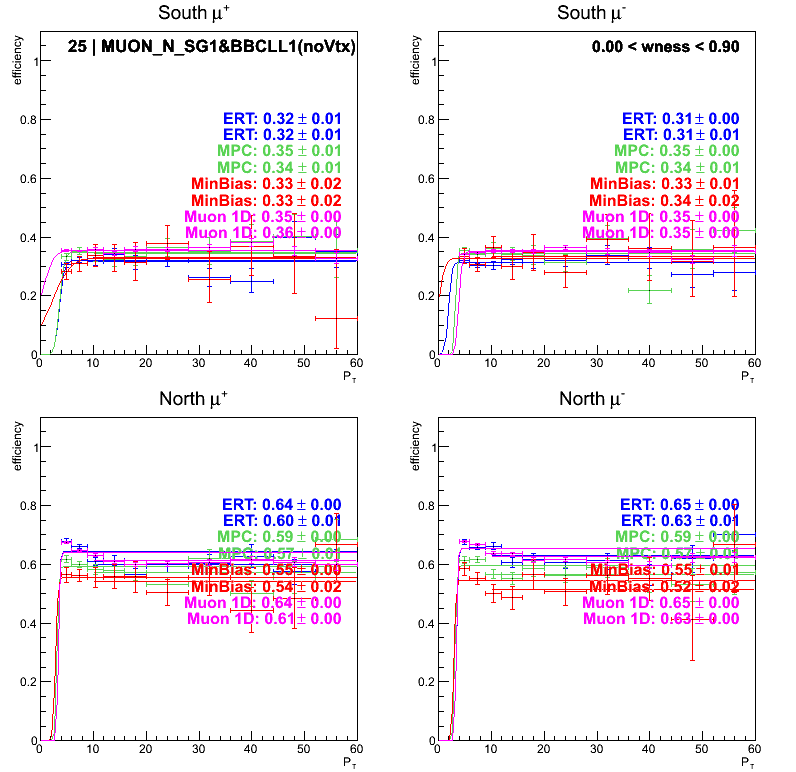
\includegraphics[width=0.5\textwidth]{./figures/run13_trigeffipt_iw0_trig25_lin.png}
  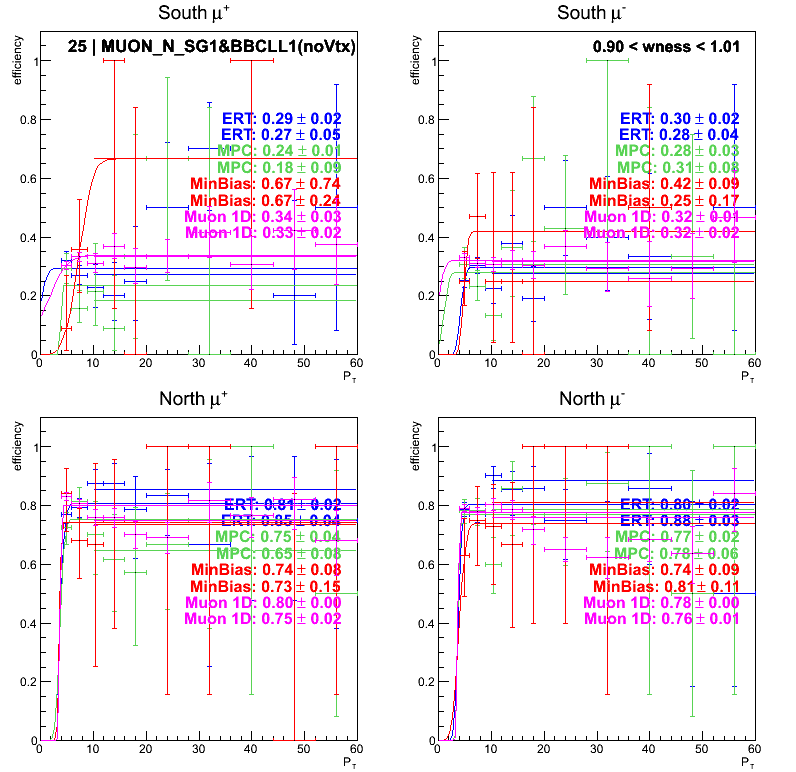
\includegraphics[width=0.5\textwidth]{./figures/run13_trigeffipt_iw1_trig25_lin.png}
  \caption{
    Left: Trigger efficiencies for trigger bit 25 (MUON\_N\_SG1\&BBCLL1(noVtx))
    for single $W$ $\rightarrow \mu$ candidatesfor the $W_{ness}$ ranges  $ 0
    \leq W_{ness} < 0.9 $ (left plot) and $W_{ness} > 0.9$. Right: The triggers
    are shown as a function of $p_T$. The efficiencies for ERT
    (blue), MPC (green), MinBias(red) and 1D (purple) triggered data samples are
    shown as well as a constant fit over the whole range~\cite{Seidl2014}.
  }
  \label{fig:run13_trigeffiptlowhighpt} 
\end{figure}

\clearpage
\subsection{Efficiencies Versus $W_{ness}$}

Next, the trigger efficiencies are evaluated as a function of the $W_{ness}$ for
$p_T$ above 5 GeV and in three rapidity bins: $1.1 < \eta < 1.4$, $1.4 < \eta <
2.0$ and $2.0 < \eta < 2.6$. The data is partitioned in $W_{ness}$ between 0,
0.1,0.3, 0.5, 0.7, 0.9 and 1. Results are summarized in
Figure~\ref{fig:run13_trigeffisn_eta0_nper0_trig17_lin}, with remaining
partitions presented in the appendix in
Figures~\ref{fig:run13_trigeffisn_eta1_nper0_trig17_lin} through
\ref{fig:run13_trigeffisn_eta1_nper0_trig27_lin}.

\begin{figure}[ht]
  \centering
  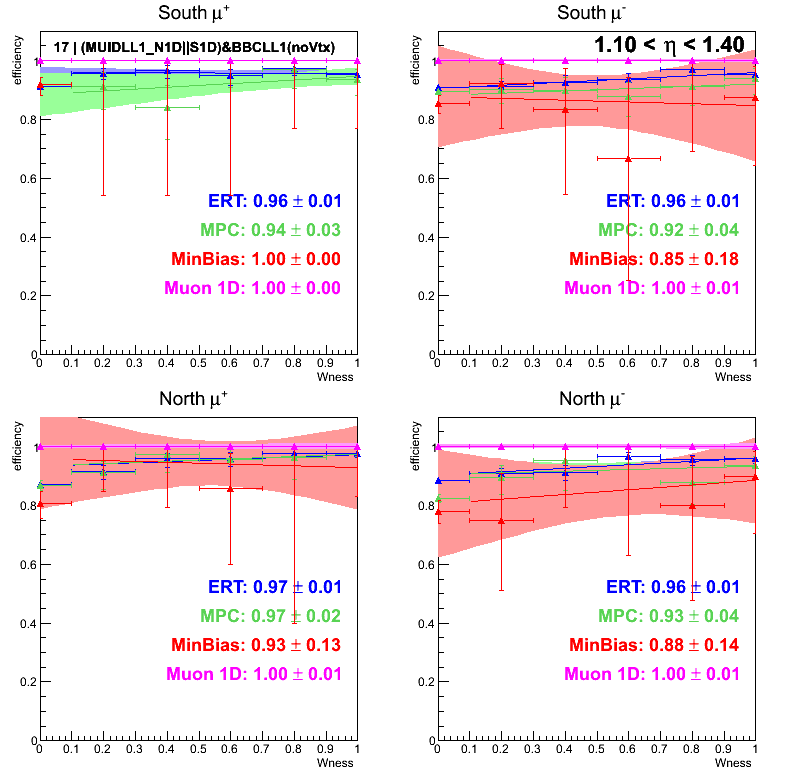
\includegraphics[width=0.8\textwidth]{./figures/run13_trigeffisn_eta0_trig17_lin.png}
  \caption{
    Trigger efficiencies for trigger bit 17
    ((MUIDLL1\_N1D$\|$S1D)\&BBCLL1(noVtx)) for single $W$ $\rightarrow \mu$
    candidates in the rapidity range $ 1.1 < \eta < 1.4$ as a function of
    $W_{ness}$. The efficiencies for ERT (blue), MPC (green), MinBias(red) and
    1D (purple) triggered data samples are shown as well as a constant fit over
    the whole range~\cite{Seidl2014}.
  }
  \label{fig:run13_trigeffisn_eta0_nper0_trig17_lin} 
\end{figure}

A linear fit for all but the first bin has been performed with the linear term
constrained, such that the efficiency, together with the previously performed
constant fit, never exceeds the allowed range between zero and unity. The total
uncertainties of the fit including the covariance are also displayed and the
efficiencies and errors in the target region at $W_{ness}$= 0.92 have been
evaluated.  This value, and uncertainties will be the baseline of the overall
trigger efficiency to be calculated.

Another extrapolation of the actual trigger efficiencies in the actual
$W_{ness}$ region can be obtained directly from the last bin from 0.9 to 1.0.
Here, still some fake muons contribute, but their fraction is already
substantially smaller and their other characteristics are already very similar
to real high momentum muons, that this range can be trusted.  

One can see in almost all triggers and data sets an increase in efficiency as
the $W_{ness}$ increases. 

\clearpage
\section{Total Trigger Efficiencies }
The relative trigger contributions $f_{trigger}$ of
Fig.~\ref{fig:triggerrel_all} were now combined with the trigger efficiencies
for each individual trigger to obtain a total, rapidity dependent efficiency for
each arm and charge. While the rapidity binning for the relative trigger
contributions is finer, the efficiencies only in the aforementioned three
rapidity bins where taken into account and multiplied with the corresponding
relative fractions. In the case of the 1D triggered data sample the 1D trigger
efficiency as average from the ERT and MPC data samples was multiplied for
triggers which include the 1D. The total trigger efficiency per fine rapitiry
bin is calculated as follows:

\begin{equation}
\epsilon (arm,charge,\eta) = \sum_{trigger} \epsilon_{trigger}(arm,charge,matching coarse \eta bin) * f_{trigger}(arm,charge,\eta)\quad.
\end{equation}

Figure \ref{fig:totaltrigeffi_all_wpt0} displays the total efficiencies and the
breakdown into the individual trigger efficiencies in the total data sample. The
several colors display the different data samples, with black is showing the
weighted average of all arm/charge partitions, with the individual
contributions are visible as a stack. The total efficiencies were
evaluated based on the plateau value in the $p_T$ dependent trigger
efficiencies. Due to the large amount of fakes this total efficiency can be
regarded as a low momentum limit of the total efficiencies.

The same is true even stronger in Fig.~\ref{fig:totaltrigeffi_all_wpt1} where
the constant fit for $p_T$ above 10 GeV was taken as individual efficiencies. As
discussed above the corresponding efficiencies appear even lower due to the even
higher fraction of fakes. 

The more realistic total trigger efficiencies although with larger uncertainties
can be found in Figs.~\ref{fig:totaltrigeffi_all_wpt2} and
\ref{fig:totaltrigeffi_all_wpt3}, which were evaluated using either the highest
$W_{ness}$ bin or based on the extrapolation of the linear fit in $W_{ness}$.
Both of these evaluations show substantially higher total efficiencies. 

As the four arm/charge partitions show reasonably similar total efficiencies, the
maximum differences to the average may serve as an estimate on the
uncertainties. 

For the total efficiencies used in the $W$ signal to background evaluation as
well as the total $W$ cross section calculation, these two systematic
uncertainties and the statistical uncertainties will be added in quadrature. 
